\documentclass[12pt]{article}
\usepackage{graphicx}

\begin{document}
	
\title{Numerical Simulation - Assignment 2}
\author{Laura Farny}

{\centering {\Large Assignment 2\\
		
		Laura Farny\\ \par}}


\begin{abstract}
	This document shows a homework assignment for the seminar Economics and Psychology of Risk and Time.
	
\end{abstract}

\textbf {Exercise 1\\}

Calculate the certainty equivalent of the prospect (0.2,€40;0.6,€50;0.2,€30), under: \\
a) Expected utility theory with the utility function \[u(x) =x/10\] with total wealth=0. \\
b) Rank dependent utility with the utility function \[u(x) =x/10\] and \[w(p) = p^{2}\] with total wealth=0. \\
\\


\textbf {Answer Exercise 1a\\}

The expected value of the prospect is EV=0.2*40+0.6*50+0.2*30=44 and the utility given the formula \[U(x)=\sum p*u\] is 4.4.\\
The certainty equivalent (CE) is calculated by determining the value of x for which an individual is indifferent of receiving the prospect or a certain amount. In this case, since utility is given by \[U(x)=x/10\]  the CE is calculated as follows:

\[U(x)=x/10 =4.4\]
\[x=4.4*10=44=CE\]\\


\textbf {Answer Exercise 1b\\}

The rank dependent utility calculated using \(U(x)=\sum \pi *u\) and \(w(p)=p^{2}\) is as follows: \\
\(0.2^{2}*4 + (0.8^{2}-0.2^{2})*5 + (1-0.8^{2})*3 = 4.24\). \\
Given that the utility is calculated as \(u(x)=0.1*x\) , so the amount for which an individual would be indifferent between the prospect or a certain amount would be \[CE=4.24/0.1=42.2\]\\

\textbf {Graph\\}

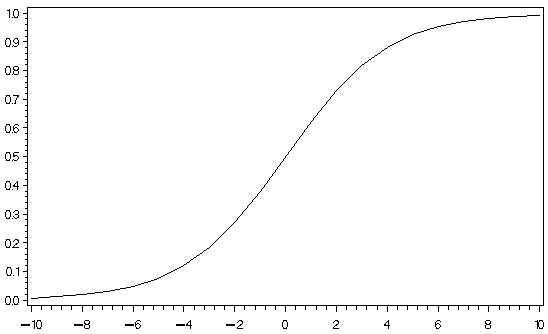
\includegraphics{graph}

\end{document}